\chapter{Running the System}
\label{app:run}

\section{Installation}

\begin{lstlisting}
python -m venv .venv
.venv\Scripts\activate              # Linux/macOS: source .venv/bin/activate
pip install -r requirements.txt     # cryptography>=47, kyber-py, ...
\end{lstlisting}

The ns-3 experiments need Linux or WSL2:
\begin{lstlisting}
pip install -r requirements.txt -r requirements-ns3.txt
\end{lstlisting}

\section{Commands}

\begin{table}[h]
\centering
\caption{Commands}
\small
\begin{tabular}{@{}p{8.6cm}p{5.4cm}@{}}
\toprule
Command & Purpose \\
\midrule
\code{python scripts/demo\_protocol.py} & the protocol step by step, with attacks \\
\code{python scripts/run\_network.py} & the 19-process distributed system \\
\code{python -m pytest} & the 55 tests \\
\code{python scripts/run\_evaluation.py} & benchmarks, attacks, consensus, figures \\
\code{python scripts/run\_ns3\_sweeps.py} & ns-3 density sweep and variants \\
\code{python scripts/run\_ns3\_sweeps.py --seeds 2 3} & extra seeds \\
\code{python scripts/make\_viewer.py} & the replay viewer (\code{results/viewer.html}) \\
\code{python scripts/make\_tables.py} & this report's tables and numbers \\
\bottomrule
\end{tabular}
\end{table}

\section{Replay viewer}

\begin{figure}[h]
\centering
\IfFileExists{../results/viewer_screenshot.png}{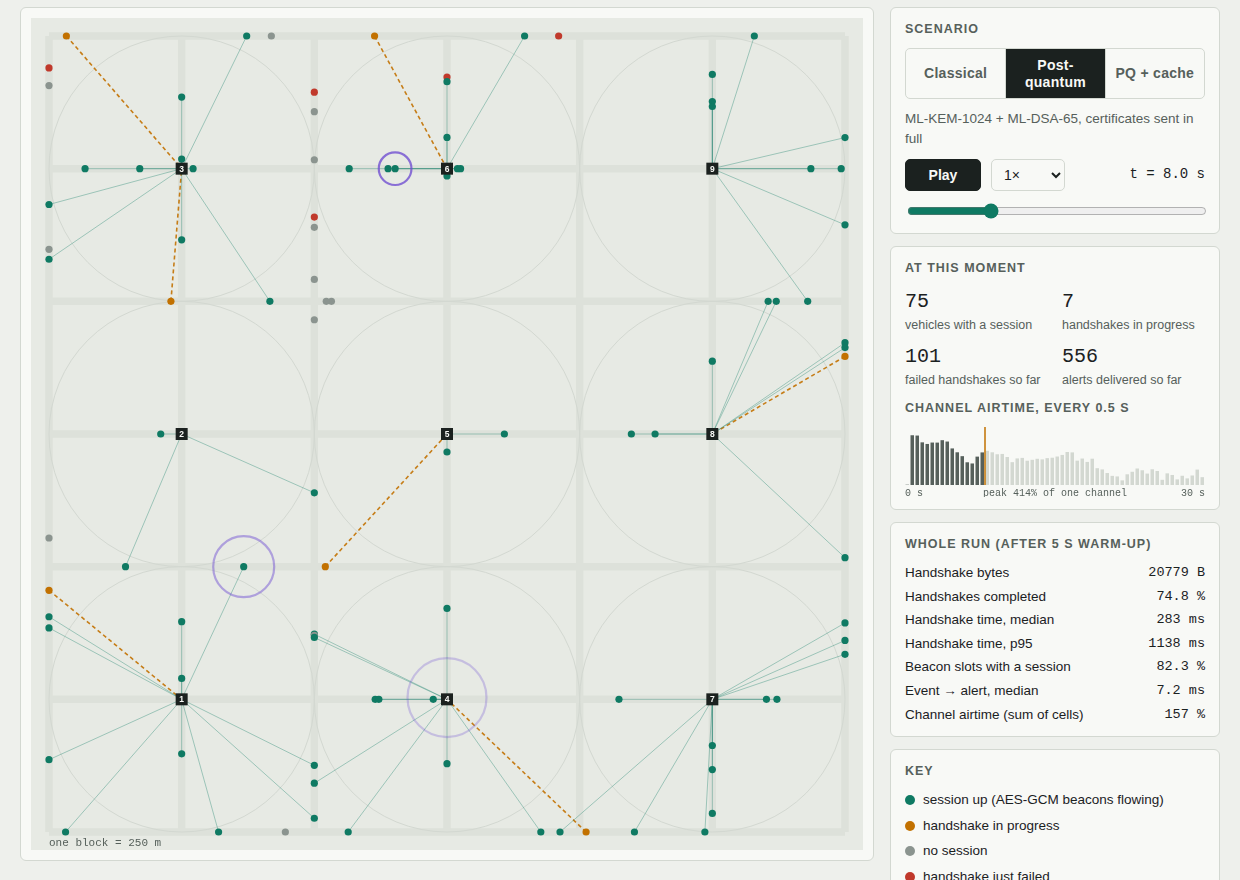
\includegraphics[width=\textwidth]{viewer_screenshot.png}}{\fbox{viewer screenshot}}
\caption{The replay viewer: vehicles (dots) on the 1.5\,km grid, RSUs (squares), handshakes in progress (dashed) and sessions (solid), with the channel airtime over time. The same run can be switched between the classical suite, DECK and DECK with certificate caching.}
\label{fig:viewer}
\end{figure}
